\documentclass[thesis.tex]{subfiles}

\begin{document}


\chapter{Other video processing tools} \label{other_video_processing_tools}
% ----------------------------------------------------------
% might remove this entire section
% ----------------------------------------------------------

We will go through some other methods not directly related to neural networks but which we think may come in handy for my thesis later on. 

\subsection{Object tracking}
%-----------------------------------------------------------
Object tracking is one of the harder problem to overcome in computer vision and is key to achieving good results in endoscopic video analysis. Tracking algorithms are developed to determine the movement of the object or objects in each video frame. The algorithm has to take into account the dynamic environment such as differences in lightning, occlusions and scaling changes. Also the absence of any prior knowledge to the object and its position further increase the complexity of the problem. \citeauthor*{DeepReinforcement17} proposed an approach for visual tracking in videos that learns to predict the bounding box locations of a target object at every frame in the paper \citetitle{DeepReinforcement17} \cite{DeepReinforcement17}. While other models depends on the capability of a CNN to learn a good feature representation for the target location in the new frame, which means that the model only tracks properly if the target lies in the spatial vicinity of the previous prediction. This is not always the case for WCE videos, where the lens of the camera can suddenly and unpredictably rotate towards the wall of the intestine. This method integrates convolutional network with recurrent network, and builds up a spatial-temporal representation of the video which means that the model is able to predict the target object's location over time.

\begin{figure}[H] % fig:object-tracking
  \begin{center}
    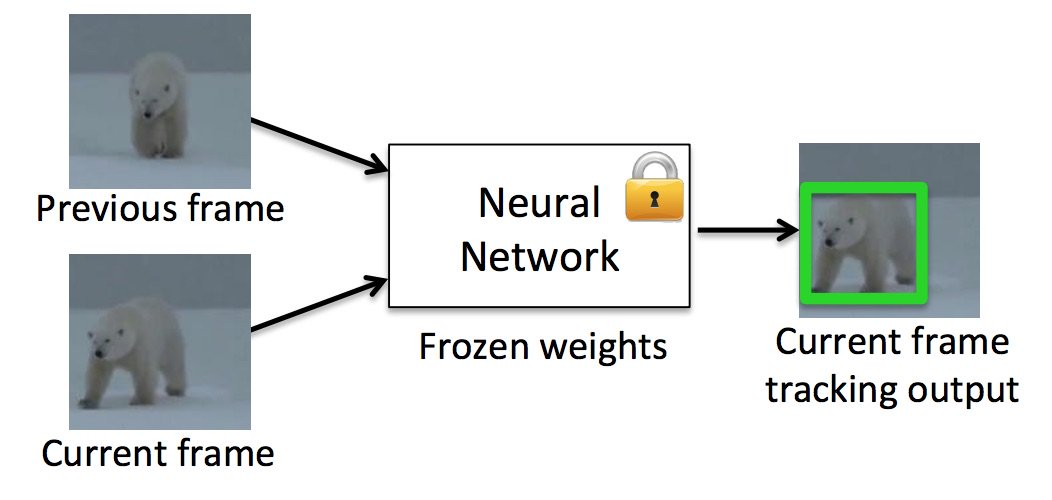
\includegraphics[width=0.7\textwidth]{object-tracking.jpg}
    \caption[Image]{Illustration of how object in two frames is tracked with a bounding box\footnotemark. }
    \label{fig:object-tracking}
  \end{center}
\end{figure}

\footnotetext{
\url{https://www.learnopencv.com/goturn-deep-learning-based-object-tracking/}
}

Our hope is that by implementing an object-tracking algorithm we can use it to classify irregularities in the colonoscopy video, and then track that object in the later frames until it disappear out of frame. This will hopefully help with reducing the robustness of the network so that the classifier will not have to check every frame for irregularities. 



\subsection{Segmentation} \label{segmentation}
%-----------------------------------------------------------
% Image/video segmentation. Specially related to the paper "U-Net: Convolutional Networks for Biomedical Image Segmentation" citekey UNetConvolutional15
Image segmention is the process of partitioning a image into multiple segments of pixel, usually each segment describing some feature of the image or an entire object or class of objects. The goal of segmentation is to simplify the image and make it easier to analyze or further process. \citeauthor*{UNetConvolutional15} propose a method in the paper \citetitle*{UNetConvolutional15} \cite{UNetConvolutional15} for using a network and training strategy that relies on the strong use of data augmentation to use the available labeled samples more effieciently. This network outperform the old method of sliding-window-convolution by a great deal. They extend the "fully convolutional network" \cite{FullyConvolutional15} such that it works with very few training images and yields more precise segmentations. The way this is achieved is to supplement a contracting network by successive layers, where instead of using pooling operators, upsampling operators are used. This means that these successive layers increase the resolution of the output. The high resolution features from the contracting path are combined with the upsampled output to localize objects and with that a convolution layer can then learn to produce more precise output based on this information. 

Another important feature in this architecture is that in the upsampling portion of the network there is also large number of feature channels. These channels allow the network to pass on context information to the higher resolution layers. 

A common problem in training neural networks are too little labeled training data. This is also the case for us. We require a lot of medical data, and personell with the expertise to correctly label our data are of high demand and they usually have very little time for projects like these. This is why \citeauthor*{UNetConvolutional15} use different methods of data augmentation to generate more training data. They apply elastic deformations to the available images, and this allows the network to learn invariance to such deformations without the need to see these transformations in the annoted image corpus. Which is particular important in biomedical segmentation since deformation used to be the most common variation in tissue and realistic deformations can be simulated efficiently \cite{UNetConvolutional15}. By doing this \citeauthor*{UNetConvolutional15} were able to achieve very good results (Table \ref{tab:segmentation_results}).

\begin{table} % table:segmentation_results
  \centering
  \begin{tabular}{ l l l }
  	\hline
    Name &				PhC-U373 &			DIC-HeLa 		\\
    \hline
    IMCB-SG (2014) &	0.2669 & 			0.2935 			\\
    KTH-SE (2014) &		0.7953 & 			0.4607 			\\ 
    HOUS-US (2014) &	0.5323 & 			- 				\\ 
    second-best 2015 &	0.83 & 				0.46 			\\
    u-net (2015) &		\textbf{0.9203} & 	\textbf{0.7756} \\
    \hline
  \end{tabular}
  \caption{Segmentation results on the ISBI cell tracking challenge in 2015.}
  \label{tab:segmentation_results}
\end{table}


\subsection{Mapping} \label{mapping}
%-----------------------------------------------------------
% Mapping of the intestine. Specially related to the paper "Deep EndoVO: A recurrent convolutional neural network (RCNN) based visual odometry approach for endoscopic capsule robots" citekey DeepEndoVO18
As mentioned in section \ref{wireless_capsule_endoscopy}, a concern when processing the images taken with a WCE is not having the spatial data you get when using a normal fiber-optic endoscope. This is why \citeauthor*{DeepEndoVO18} has recently made substantial progress in converting passive capsule endoscopes to active capsule robots, enabling more accurate, precise, and intuitive detection of the location and size of the diseased areas by developing reliable real time pose estimation functionality of the capsule with RCNN's\footnote{Deep recurrent convolutional neural networks} \cite{DeepEndoVO18}. See Figure \ref{fig:deep_endovo_example} for an example.

This architecture uses inception modules for feature extraction and a RNN for sequential modelling of motion dynamics to regress the robot's orientation and position in real time. By taking multiple of RGB Depth images with timestamps it can calculate the 6-DoF pose of the capsule without the need of any extra sensors. For obtaining the depth images \citeauthor*{DeepEndoVO18} use the shape from shading (SfS) technique of \citeauthor{ShapeShading94} \cite{ShapeShading94}. This model outperforms state-of-the-art models like LSD SLAM and ORB SLAM.

\begin{figure}[h] % fig:deep_endovo_example
  \centering
  \begin{subfigure}[b]{0.4\linewidth}%
    \centering
    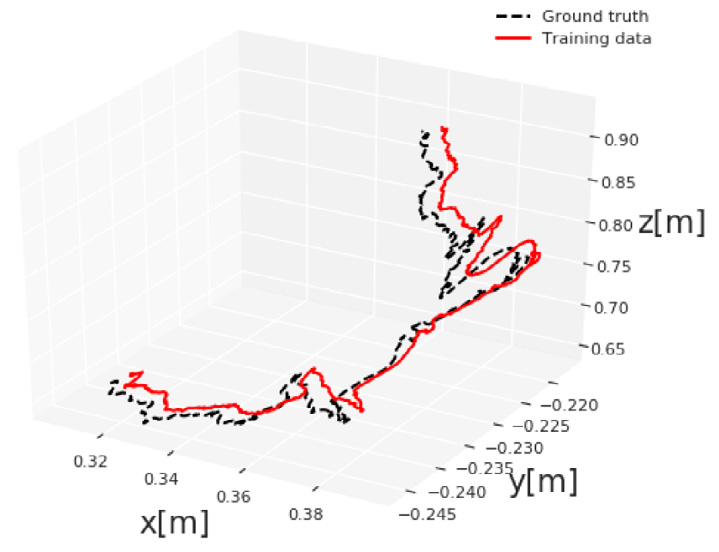
\includegraphics[width=\linewidth]{endovo_training_data}%
    \caption{Training data vs ground truth. }%
    \label{fig:endovo_training_data}%
  \end{subfigure}%
  \quad
  \begin{subfigure}[b]{0.4\linewidth}%
    \centering
    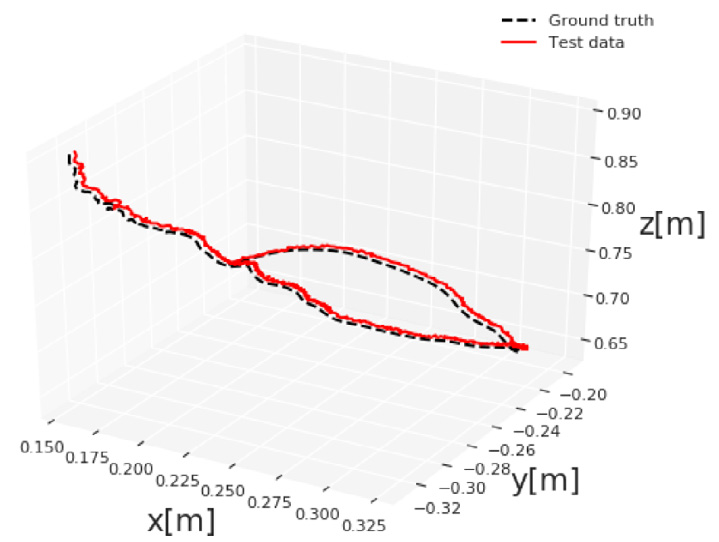
\includegraphics[width=\linewidth]{endovo_test_data}%
    \caption{Test data vs ground truth. }%
    \label{fig:endovo_test_data}%
  \end{subfigure}%
  \caption{An example of Deep EndoVO accuracy \cite{DeepEndoVO18}. }%
  \label{fig:deep_endovo_example}%
\end{figure}%


\end{document}